%%%%%%%%%%%%%%%%%%%%%%% file template.tex %%%%%%%%%%%%%%%%%%%%%%%%%
%
% This is a general template file for the LaTeX package SVJour3
% for Springer journals.          Springer Heidelberg 2010/09/16
%
% Copy it to a new file with a new name and use it as the basis
% for your article. Delete % signs as needed.
%
% This template includes a few options for different layouts and
% content for various journals. Please consult a previous issue of
% your journal as needed.
%
%%%%%%%%%%%%%%%%%%%%%%%%%%%%%%%%%%%%%%%%%%%%%%%%%%%%%%%%%%%%%%%%%%%
%
% First comes an example EPS file -- just ignore it and
% proceed on the \documentclass line
% your LaTeX will extract the file if required
\begin{filecontents*}{example.eps}
%!PS-Adobe-3.0 EPSF-3.0
%%BoundingBox: 19 19 221 221
%%CreationDate: Mon Sep 29 1997
%%Creator: programmed by hand (JK)
%%EndComments
gsave
newpath
  20 20 moveto
  20 220 lineto
  220 220 lineto
  220 20 lineto
closepath
2 setlinewidth
gsave
  .4 setgray fill
grestore
stroke
grestore
\end{filecontents*}
%
\RequirePackage{fix-cm}
%
%\documentclass{svjour3}                     % onecolumn (standard format)
%\documentclass[smallcondensed]{svjour3}     % onecolumn (ditto)
\documentclass[smallextended]{svjour3}       % onecolumn (second format)
%\documentclass[twocolumn]{svjour3}          % twocolumn
%
\smartqed  % flush right qed marks, e.g. at end of proof
%
\usepackage[latin1]{inputenc}
\usepackage{graphicx}
\usepackage{color}
\usepackage{url}
\usepackage[english]{babel}
%
% \usepackage{mathptmx}      % use Times fonts if available on your TeX system
%
% insert here the call for the packages your document requires
%\usepackage{latexsym}
% etc.
%
% please place your own definitions here and don't use \def but
% \newcommand{}{}
%
% Insert the name of "your journal" with
% \journalname{myjournal}
%
\begin{document}

\title{Creating Autonomous Agents for Playing Super Mario Bros Game by Means of Evolutionary Finite State Machines}
%\subtitle{Do you have a subtitle?\\ If so, write it here}

\titlerunning{Creating Autonomous Agents for Super Mario Game with Evolutionary FSMs}        % if too long for running head

\author{A.M. Mora \and M.S. Rodr�guez-Domingo \and R.M. Hidalgo-Berm�dez \and  J.J. Merelo \and P. Garc�a-S�nchez \and P.A. Castillo}

\authorrunning{A.M. Mora et al.} % if too long for running head

\institute{A.M. Mora, M.S. Rodr�guez-Domingo, R.M. Hidalgo-Berm�dez, \\
J.J. Merelo, P. Garc�a-S�nchez, P.A. Castillo\at
Departamento de Arquitectura y Tecnolog�a de Computadores. \\
ETSIIT-CITIC. \\
University of Granada, Spain. \\
              Tel.: +34-958241778\\
              Fax: +34-958248993\\       \email{\{amorag,jmerelo,pgarcia,pedro\}@geneura.ugr.es\\
       rosa.hb84@gmail.com, zandri@gmail.com}           %  \\
%             \emph{Present address:} of F. Author  %  if needed
%           \and
%           S. Author \at
%              second address
}

\date{Received: date / Accepted: date}
% The correct dates will be entered by the editor

\maketitle

\begin{abstract}
This paper proposes the design and improvement of an autonomous agent based in a mixture between behavioural models (Finite State Machines, FSMs) and evolutionary methods (Genetic Algorithms in this case), consisting in the consideration of FSMs as part of the individuals to evolve. This leads to finally obtain a so-called \textit{bot}, which is able to autonomously complete different scenarios on a simulator of Super Mario Bros. game. The bot should follow \textit{Gameplay} track rules of the international Mario AI Championship.
Mono- and multi-seed approaches (evaluation in one play or multiple plays respectively) have been analysed, considering the machine resources consumption, which turns in a bottleneck in some experiments. However, the methods yield agents which can finish levels of different difficulties successfully, and which play much better than an expert human player. These agents would have an excellent performance in they would participate in this competition track.
\keywords{Videogames \and Super Mario Bros \and Artificial Intelligence \and \and Genetic Algorithms \and Finite State Machines \and Autonomous Agents \and Non Player Characters \and Bots}
% \PACS{PACS code1 \and PACS code2 \and more}
% \subclass{MSC code1 \and MSC code2 \and more}
\end{abstract}

%
%%%%%%%%%%%%%%%%%%%%%%%%%%%%%%%   INTRODUCTION   %%%%%%%%%%%%%%%%%%%%%%%%%%%%%%%
%
\section{Introduction}
\label{sec:intro}

Videogames have considerably evolved from their original concept to the complex technological products that they have become, creating a massive industry and market as important as the cinematographic one. Thus, in recent years, most of the game development has been focused on the technical part (graphics and sound), leaving the Artificial Intelligence (AI) aside. However, nowadays artificial intelligence (specifically Computational Intelligence, CI) is becoming more relevant, since videogames players are requesting for opponents which mean a real challenge, and so provide a better gaming experience. This is leading to new research lines on how to create non-playing characters with adapted and unpredictable behaviour, i.e. more human-like in some sense.

Going back to the first modern video games, and focusing on one of the most prolific characters, in 1981 Shigeru Miyamoto\footnote{Designer and producer of Nintendo Ltd., and winner of the 2012 Pr�ncipe de Asturias Prize in Humanities and Communication} created Donkey Kong, in which a plumber named Jumpman tries to rescue his girlfriend from a gorilla. This character was evolved, and in 1983 (thanks again to Shigeru Miyamoto) Mario Bros. games series appeared. The most famous was platform game Super Mario Bros., which was launched in arcade and also in the Nintendo's home console NES. Several other sequels have been published, including the blockbuster Super Mario World in the 90s, which presented a great improvement in graphics, sound and playability.

All these games present the plumber Mario who must rescue the princess of Mushroom Kingdom, Peach, kidnapped by the king of the koopas, Bowser. The gameplay consists in moving across lateral platforming levels, trying to avoid different types of enemies and obstacles and using some items, such as mushrooms (Mario grows) or fire flowers (Mario can shot). 

Videogames have become one of the most extended research areas regarding the Artificial Intelligence (AI) field, yielding the so-called Computational Intelligence (CI) branch. Several games have become extended frameworks for study new techniques and algorithms in these scopes, such as Quake \cite{laird2001using}, Unreal \cite{Agent_Smith_CEC2009,cooperativebots_CIG2010}, Pac-Man \cite{Pac-MAnt_CIG2010,MTCS_PacMan}, Starcraft \cite{starcraft_bayesianmodel,potfields_starcraft} and, of course, the commented Super Mario Bros. \cite{SuperMario_playerexperience,SuperMario_Togelius,SuperMario_rulebased,SuperMario_levelgeneration}.

Thus, there exists a framework developed for the latter called \textit{Mario AI}, a modified version of the game known as Infinite Mario Bros.\footnote{\url{http://www.mojang.com/notch/mario/}}, an open source application where the researchers can implement, for instance interactive and autonomous behavioural routines (or agents), using the set of functions and variables it offers.
Moreover, there is an additional motivation for the scientific community to perform these studies, which is the competition \textit{Mario AI Championship}\footnote{\url{http://www.marioai.org/}}, held three times a year, inside several famous CI conferences and workshops. There are some tracks in it: Learning, Level generation, Turing test, and Gameplay.
The latter is devoted to create an autonomous agent, also called \textit{bot}, which must perform the best as possible in automatically playing and pass sequential levels with a growing difficulty.

This work in enclosed in this track, and presents different approaches of autonomous agents, which follow the behaviour modelled by means of a Finite State Machine (FSM) \cite{FSM_Booth}. This behavioural engines are generated as part of the individuals in the population of an Evolutionary Algorithm (EA) \cite{EAs_Back96}, starting from simple states and combining them to create wide sets of outputs in every state. Thus, this is a shape of evolutionary FSMs, which is, to our knowledge, a novel approach inside this scope.

This EA, a Genetic Algorithm (GA) \cite{GAs_Goldberg89}, has been applied offline (not during game), as have been done in many CI researches in the videogames scope \cite{evolutionary_learning-offline,Mora_Unrealbot_EVO2010,ControllingBot_CEC2010,Genebot_CEC11}.
Two different approaches have been considered, mainly experimenting with different evaluation schemes, being: 
\begin{itemize}
    \item a \textit{mono-seed} evaluation, in which every individual plays just one level/scenario and just one time. Once it has finished the level, died, or got stacked, its performance is evaluated.
    \item a \textit{multi-seed} evaluation, which considers 30 plays in 30 different levels/scenarios (generated with different randomisation seed). This approach tries to obtain more general agents, which can pass any situation in a level.
\end{itemize}

The approaches have been widely tested and analysed, getting an optimal set of parameters for the EA and thus, very competent agents in a number of difficulty levels, which could participate successfully in the competition. However, these approaches (much more multi-seed) demand a high amount of computation resources and machine memory, which means it is not possible to optimise in any difficulty level, due to the huge amount of inputs, rules and outputs to consider in the evolution.

The rest of the paper is organised as follows. Next section presents some preliminary concepts and background of the work. Section \ref{sec:environment} defines the problem itself, describing the Infinite Mario Bros. platform, along with the competition rules, regarding the main features that the agent must consider and its constraints. Then, Section \ref{sec:FSMagent} introduces the agents' approaches which will be analysed in the paper, along with the set of experiments conducted to perform this analysis in Section \ref{sec:experiments}. Finally, Section \ref{sec:conclusions} describes the reached conclusions and proposes some future lines of work.

%
%%%%%%%%%%%%%%%%%%%%%%%%%%%%%%%   BACKGROUND  %%%%%%%%%%%%%%%%%%%%%%%%%%%%%%%
%
\section{Preliminary concepts and background}
\label{sec:preliminaryconcepts}

In this section, the main techniques applied in the development of this work are briefly described.

%----------------------------------------------------------------------------
\subsection{Genetic Algorithms}
\label{subsec:GAs}

Evolutionary Algorithms (EAs) \cite{EAs_Back96} are a class of direct, probabilistic search and optimisation algorithms gleaned from the model of darwinistic evolution. They have been widely used for solving combinatorial and optimisation problems. 
An EA works with a population of possible solutions (individuals) for the target problem, a selection method that favours better solutions and a set of operators that act upon the selected solutions. After an initial population is created (usually randomly), the selection and operators are successively applied to the individuals in order to create new populations that replace the older one. This process guarantees that the average quality of the individuals tends to increase with the number of generations. Eventually, depending on the type of problem and on the efficiency of the EA, an optimal solution may be found.
The most extended class of EA are the Genetic Algorithms (GAs) \cite{GAs_Goldberg89}. A GA is composed of a \textit{population of candidate solutions} to a problem that evolve towards optimal (local or global) points of the search space by recombining parts of the solutions to generate a new population. The decision variables of the problem are encoded in strings with a certain length and cardinality. In GAs' terminology, these strings are referred to as \textit{chromosomes}, each string position is a \textit{gene} and its values are the \textit{alleles}. The alleles may be binary, integer, real-valued, etc, depending on the codification (which in turn may depend on the type of problem). 
As stated, the ``best'' parts of the chromosomes (or building-blocks) are guaranteed to spread across the population by a \textit{selection mechanism} that favours better (or fitter) solutions. The quality of the solutions is evaluated by computing the \textit{fitness} values of the chromosomes; this fitness function is usually the only information given to the GA about the problem. 
A standard GA's procedure is shown in Figure \ref{fig:GA_pseudocode}.

\begin{figure}[ht]
\begin{center}
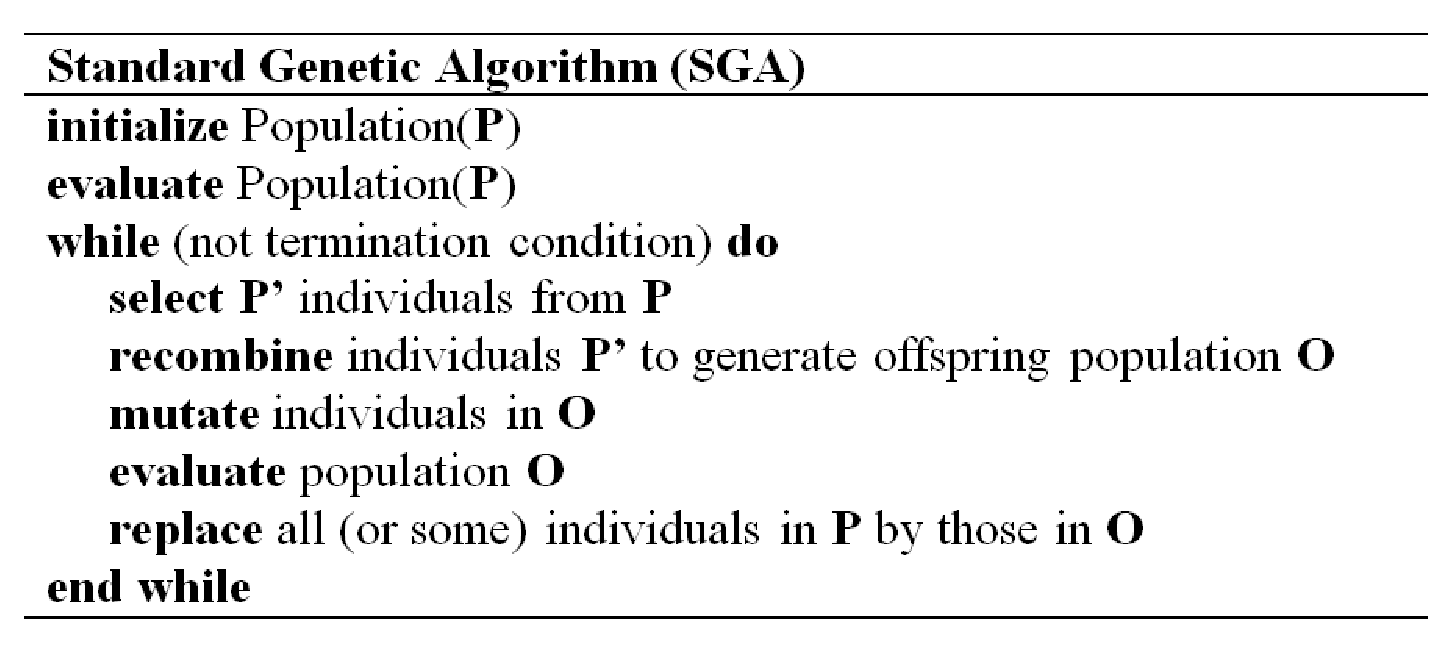
\includegraphics[scale=0.45]{imags/GA_pseudocode.eps}
\caption{Standard GA pseudocode.
\label{fig:GA_pseudocode}}
\end{center}
\end{figure}

It works as follows: First, a population of chromosomes is randomly generated. All the chromosomes in the population are then evaluated according to the fitness function. A pool of parents (or mating pool) is selected by a method that guarantees that fitter individuals have a better chance of being in the pool. After selection, a new population is generated by recombining the genes in the parents' population. This is usually done with a crossover operator (1-point crossover, or uniform crossover, amongst many proposals that can be found in the Evolutionary Computation literature) that recombines the genes of two parents and generates two offspring according to a crossover probability. Then, once the offspring population is complete, the new chromosomes are mutated before being evaluated by the fitness function. Mutation operates at gene level considering a probability (which is usually very low).
After the evaluation of the offspring population the algorithm starts the replacement of the old population, following a specific policy. Generational replacement, for instance, replaces the old population by the offspring. A steady-state strategy, on the other hand, will replace a fraction (typically, two individuals) of the old population by the best individuals in the offspring population. Normally, an $e$-elitism strategy is used, i.e., the best $e$ chromosomes from the old population are copied without mutation to the new population. The remaining individuals are selected according to any method. 
This process goes on until a stop criterion is met. Then, the best individual in the population is retrieved as a possible solution to the problem. 

EAs have been applied in a wide range of optimisation problems, including in recent years (10 years ago) their application in videogames area \cite{optimalRTS,tactics_evolutionary_learning,SuperMario_Togelius,Agent_Smith_CEC2009,cooperativebots_CIG2010}. The problem is they usually involve considerable computational cost and thus they are not frequently used in real-time. In fact, the most successful proposals for using EAs in games correspond to offline applications \cite{evolutionary_learning-offline,Mora_Unrealbot_EVO2010,Genebot_CEC11}, that is, the EA works (for instance, to improve the operational rules that guide the bot's actions) while the game is not being played, and the results or improvements can be used later during the game. Through offline evolutionary learning, the quality of bots' intelligence in commercial games can be improved, and this has been proven to be more effective than opponent-based scripts.
This way, in this work, an offline EA is applied to a parametrised behavioural model for a Super Mario agent, in order to improve its decision engine, which will be used later during game.

%----------------------------------------------------------------------------
\subsection{Finite State Machines}
\label{subsec:FSMs}

A Finite State Machine (FSM) \cite{FSM_Booth} or Finite State Automaton is a computational model which represents a set of \textit{states} and connections between them. Every connection correspond to a \textit{transition} from one state to another one, depending on the state inputs and the so-called transition function.

\begin{figure}[ht]
\begin{center}
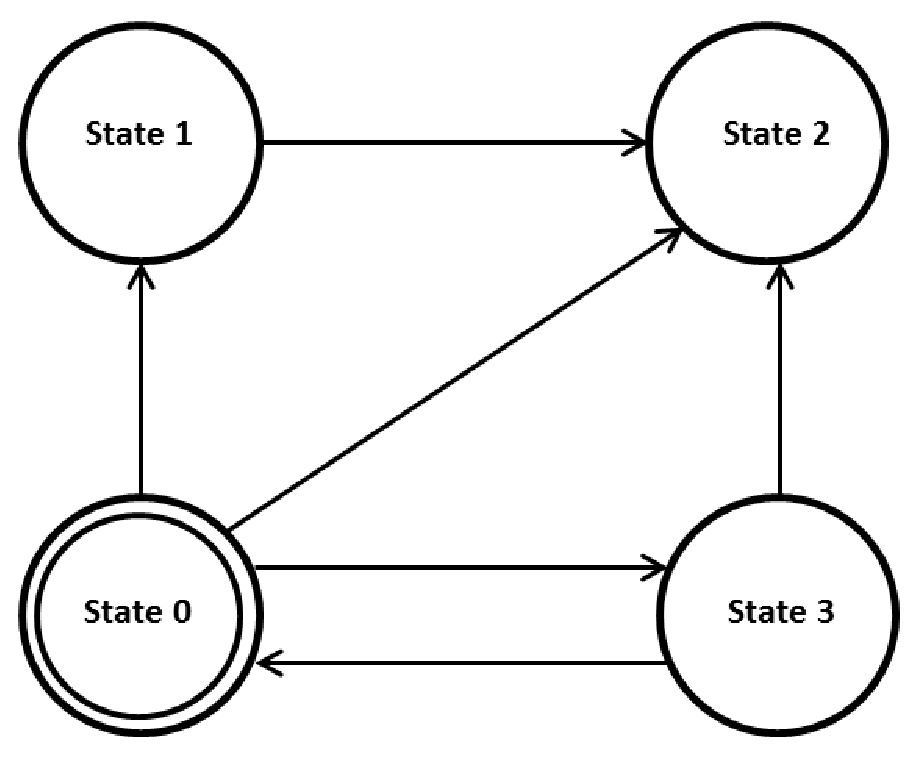
\includegraphics[scale=0.45]{imags/example_fsm.eps}
\caption{Example of FSM with four states (circles) and some transitions between them (directed arcs).
\label{fig:example_fsm}}
\end{center}
\end{figure}

It is represented as a directed graph (see Figure \ref{fig:example_fsm}), where the states are nodes labelled with a name, and the transitions are edges with an associated value representing the input that should be received to move between states through this transition. The graph can be connected at different degrees (is not always fully connected), depending on the possible transitions to model.

There is usually an initial state, where the model starts working, and a final state, which is the final output of the automaton.

FSMs were initially designed to recognise regular and formal languages, but nowadays they are used as a powerful behaviour modelling tool inside videogames, i.e., the AI of an autonomous character can be defined by means of a FSM. 
They are based in \textit{sensors}, which receive environmental inputs and \textit{actuators}, which perform the response actions to these inputs. In the FSM model, the possible values received by the sensors are set in the edges of the graph (as transitions), meanwhile the actuators' actions happen in every state.
Several videogames have implemented this technique, from Pac-Man (modelling the ghosts' behaviour) to Unreal Tournament series, which is one of the best considered games regarding its Bots (agents) AI.

In the present work, the behavioural model for our Mario agent has been implemented by means of a FSM, since it can easily model (or simulate) the behaviour of an expert player.


%%%%%%%%%%%%%%%%%%%%%%%%%%%%%  ENVIRONMENT %%%%%%%%%%%%%%%%%%%%%%%%%%%%%%%%

\section{Mario AI: Environment and Competition}
\label{sec:environment}

%---------------------------------------------------------------------

\subsection{The Environment}
\label{subsec:environment}

The game consists in moving the character, Mario, through bi-dimensional levels. He can move left and right, down (crouch), run (letting the button pushed), jump and shoot fireballs (when in ``fire'' mode).

The main goal is complete the level, whereas secondary goals could be  killing enemies and collecting coins or other items. These items may be hidden and may cause Mario to change his state (for instance a fire flower placed `inside' a block).
The difficulty of the game lies in the presence of cliffs/gaps and enemies. Mario loses power (i.e., its status goes down one level) when touched by an enemy, and dies if he falls off a cliff or if he is touched in the smaller state. Figure \ref{fig:mario_environment} (left) shows a screen capture of the game.

\begin{figure}
\begin{center}
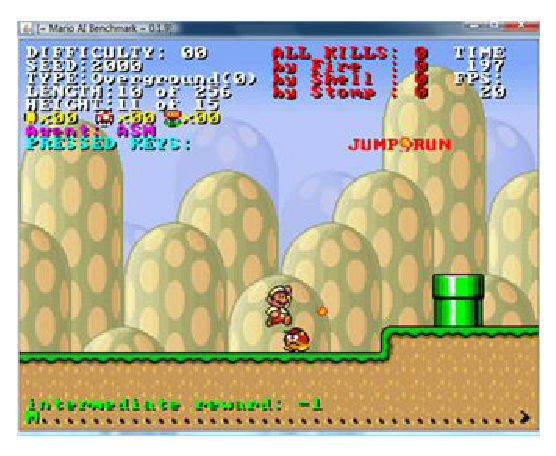
\includegraphics[scale=0.63]{imags/level_example.eps}
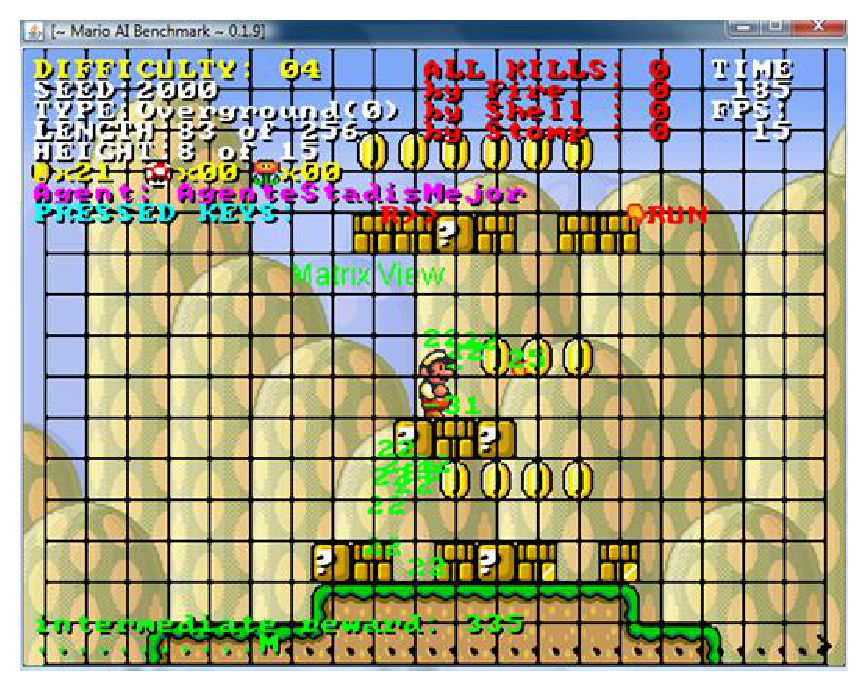
\includegraphics[scale=0.4]{imags/mario_matrix.eps}
\caption{Infinite Mario screen capture showing a level, and the information provided by the Mario AI simulator.
\label{fig:mario_environment}}
\end{center}
\end{figure}

Mario can be in three different modes:

\begin{itemize}
\item {\em Small}: In this mode Mario is smaller than in the others. If an enemy strikes him, Mario dies. He can't crouch.
\item {\em Big}: This is Mario's intermediate mode. Mario reaches this mode if he is in Fire state and an enemy touches him, or devouring a mushroom in the Small state.
\item {\em Fire}: In it Mario can shoot fireballs. Mario can reach this mode if he is in Big mode and takes a fire flower.
\end{itemize}

The simulator provides information about Mario's surrounding areas (See Figure \ref{fig:mario_environment} (right)). According to the rules of the competition, two matrices give this information, both of them are 19x19 cells size, centred in Mario. One contains the positions of surrounding enemies, and the other provides information about the objects in the area (scenery objects and items).

Every tick (40 ms), Mario's next \textit{action} must be indicated. This action consist in a combination of the five possible movements that Mario can do (left, right, down, fire/speed, jump). This information is encoded into a boolean array, containing a true value when a movement must be done.

The action to perform depends, of course, of the scenery characteristics around Mario, but it is also important to know where the enemies are and their type. Thus, the agent could know if it is best to jump, shoot or avoid them. We have defined four main enemies groups according to what the agent needs to do to neutralise them: 
%one for enemies who die by a fireball/jump/Koopa shell, other for those who only die by a fireball, others which only die jumping on them, and finally others which just die by a Koopa shell.
%
\begin{itemize}
\item Enemies who can die by a fireball strike or if Mario jumps on them and crushes them or if Mario is carrying a koopa shell and throws it at the enemies: Goomba, Goomba Windged, Green Koopa, Red Koopa, Koopa Windged Green, Red Koopa Windged.

\item Enemies who only die by a fireball strike: carnivorous flowers that appear in the pipes.

\item Enemies who only die when Mario jumps on them and crushes them: the cannon balls.

\item Enemies who only die if Mario launches a koopa shell against them: the Spiky and Spiky Windged.
\end{itemize}

%---------------------------------------------------------------------

\subsection{The Competition}
\label{subsec:competition}

The proposed agents follow the rules of the Mario AI Championship\footnote{\url{http://www.marioai.org/}} devoted to address different CI tasks (commented in the following paragraph).

Specifically, Mario AI is a simulator, a version of Infinite Mario Bros., which is available in open source and make it easier for the competitors to implement their algorithms, using a set of classes, variables and high-level functions.
It includes a wide support for implementing autonomous agents to control Mario character using AI techniques.

The competition consists of four categories: 
\begin{itemize}
    \item Gameplay: looking for the best Mario agent (bot), i.e. the one who can pass a higher amount of levels with growing difficulty.
    \item Learning: the agent must learn to play a particular level in a limited time.
    \item Level Generation: generation of levels which should be as fun as possible (according to human players).
    \item Turing Test: the agent must behave as a human.
\end{itemize}

Even being a relatively new competition, it has already been quite successful and had numerous participants with very interesting results and algorithms. For example the work by Bojarski and Bates-Congdon, called REALM \cite{SuperMario_rulebased}, in which an agent based on a evolutionary set of rules is developed, specifying some goals to achieve starting from a set of conditions and actions. This agent won the competition in the categories of Gameplay and Learning in the CIG 2010 edition.

In the category of Gameplay the main goal is to complete as many levels as possible. The problem can be interpreted as a pathfinding one, as Baumgarten \cite{SuperMario_Astar} did. He solved the objective of finding the fastest way through the surroundings in which Mario stays alive by means of an A* searching. This algorithm has proved to be quick and flexible enough to find routes through the generated levels even in real-time.

Our aim has been implementing an intelligent agent which could compete in the Gameplay track. In order to do this, we have applied GAs along with behavioural models (set of rules and a FSM).
The choice of Genetic Algorithms is due to its adaptability, as with them we do not need specific knowledge of the problem that we want to solve; they operate with diverse simultaneous solutions to the problem, and they allow to optimise these solutions with regard to different goals. Even though its convergence will not be as fast as that of other more specific algorithms for the problem, that we want to tackle, in most of the cases we will find a solution which, even though it is not the best possible, it will be the best for the pre-established aims.

%%%%%%%%%%%%%%%%%%%%%%%%%%%%%  AGENT DESIGN %%%%%%%%%%%%%%%%%%%%%%%%%%%%%%%%

\section{Evolutionary FSM-based Agents}
\label{sec:FSMagent}

We have named the objective agent to obtain \textit{evoFSM-Mario}, since it is based in a FSM which models a logical behaviour, such as expert player knowledge.
This tool has been combined with EAs (GAs), given their excellent adaption and optimisation capabilities, which are very useful for improving predefined behavioural rules.

The FSMs will model a set of limited states for the agent, which correspond to all the possible (valid) actions an agent can perform in a specific moment, i.e. feasible combinations of Mario's basic movements and actions, i.e. moving left, moving right, crouch (going down), jump and fire/run.
Table \ref{tab:FSMstates} shows a proposed codification of the states in boolean values, in order to deal with them in the GA.

\begin{table} [htbp]
\caption{Codification of the feasible states of the FSM which will model the Mario agent's AI. 1 is $true/active$, 0 is $false/non-active$.
\label{tab:FSMstates} }
\centering
{\small
\begin{tabular}{|l|l|l|l|l|l|}
\cline{2-6}
\multicolumn{1}{l|}{} & \multicolumn{1}{c|}{Right} & \multicolumn{1}{c|}{Left} & \multicolumn{1}{c|}{Fire/Run} & \multicolumn{1}{c|}{Jump} & \multicolumn{1}{c|}{Down} \\ 
\hline
\textit{State 0} & \multicolumn{1}{c|}{1} & \multicolumn{1}{c|}{0} & \multicolumn{1}{c|}{0} & \multicolumn{1}{c|}{0} & \multicolumn{1}{c|}{0} \\ 
\hline
\textit{State 1} & \multicolumn{1}{c|}{1} & \multicolumn{1}{c|}{0} & \multicolumn{1}{c|}{0} & \multicolumn{1}{c|}{1} & \multicolumn{1}{c|}{0} \\ 
\hline
\textit{State 2} & \multicolumn{1}{c|}{1} & \multicolumn{1}{c|}{0} & \multicolumn{1}{c|}{1} & \multicolumn{1}{c|}{0} & \multicolumn{1}{c|}{0} \\ 
\hline
\textit{State 3} & \multicolumn{1}{c|}{1} & \multicolumn{1}{c|}{0} & \multicolumn{1}{c|}{1} & \multicolumn{1}{c|}{1} & \multicolumn{1}{c|}{0} \\ 
\hline
\textit{State 4} & \multicolumn{1}{c|}{0} & \multicolumn{1}{c|}{1} & \multicolumn{1}{c|}{0} & \multicolumn{1}{c|}{0} & \multicolumn{1}{c|}{0} \\ 
\hline
\textit{State 5} & \multicolumn{1}{c|}{0} & \multicolumn{1}{c|}{1} & \multicolumn{1}{c|}{0} & \multicolumn{1}{c|}{1} & \multicolumn{1}{c|}{0} \\ 
\hline
\textit{State 6} & \multicolumn{1}{c|}{0} & \multicolumn{1}{c|}{1} & \multicolumn{1}{c|}{1} & \multicolumn{1}{c|}{0} & \multicolumn{1}{c|}{0} \\ 
\hline
\textit{State 7} & \multicolumn{1}{c|}{0} & \multicolumn{1}{c|}{1} & \multicolumn{1}{c|}{1} & \multicolumn{1}{c|}{1} & \multicolumn{1}{c|}{0} \\ 
\hline
\textit{State 8} & \multicolumn{1}{c|}{0} & \multicolumn{1}{c|}{0} & \multicolumn{1}{c|}{0} & \multicolumn{1}{c|}{0} & \multicolumn{1}{c|}{0} \\ 
\hline
\textit{State 9} & \multicolumn{1}{c|}{0} & \multicolumn{1}{c|}{0} & \multicolumn{1}{c|}{0} & \multicolumn{1}{c|}{0} & \multicolumn{1}{c|}{1} \\ 
\hline
\textit{State 10} & \multicolumn{1}{c|}{0} & \multicolumn{1}{c|}{0} & \multicolumn{1}{c|}{0} & \multicolumn{1}{c|}{1} & \multicolumn{1}{c|}{0} \\ 
\hline
\textit{State 11} & \multicolumn{1}{c|}{0} & \multicolumn{1}{c|}{0} & \multicolumn{1}{c|}{0} & \multicolumn{1}{c|}{1} & \multicolumn{1}{c|}{1} \\ 
\hline
\textit{State 12} & \multicolumn{1}{c|}{0} & \multicolumn{1}{c|}{0} & \multicolumn{1}{c|}{1} & \multicolumn{1}{c|}{0} & \multicolumn{1}{c|}{0} \\ 
\hline
\textit{State 13} & \multicolumn{1}{c|}{0} & \multicolumn{1}{c|}{0} & \multicolumn{1}{c|}{1} & \multicolumn{1}{c|}{1} & \multicolumn{1}{c|}{0} \\ 
\hline
\end{tabular}
}

\end{table}

%\begin{table} [htbp]
%\centering
%{\footnotesize
%\begin{tabular}{|c|c|c|c|c|c|c|c|c|c|c|c|c|c|c|}
%\hline
%& \textit{St 0}  & \textit{St 1} & \textit{St 2} & \textit{St 3} & \textit{St 4} & \textit{St 5} & \textit{St 6} & \textit{St 7} & \textit{St 8} & \textit{St 9} & \textit{St 10} & \textit{St 11} & \textit{St 12} & \textit{St 13}\\
%\hline
%Right & 1 & 1 & 1 & 1 & 0 & 0 & 0 & 0 & 0 & 0 & 0 & 0 & 0 & 0\\
%\hline
%Left & 0 & 0 & 0 & 0 & 1 & 1 & 1 & 1 & 0 & 0 & 0 & 0 & 0 & 0\\
%\hline
%Fire/Run & 0 & 0 & 1 & 1 & 0 & 0 & 1 & 1 & 0 & 0 & 0 & 0 & 1 & 1\\
%\hline
%Jump & 0 & 1 & 0 & 1 & 0 & 1 & 0 & 1 & 0 & 0 & 1 & 1 & 0 & 1\\
%\hline
%Down & 0 & 0 & 0 & 0 & 0 & 0 & 0 & 0 & 0 & 1 & 0 & 1 & 0 & 0\\
%\hline
%\end{tabular}
%}
%\caption{Codification of the feasible states of the FSM which will model the Mario agent's AI. 1 is $true/active$, 0 is $false/non-active$.
%\label{tab:FSMstates} }
%\end{table}

Depending on an input string, the state changes (or remains), so the transition is decided. Inputs are the possible situations of the agent in the environment: for example, find an enemy or being near a cliff/gap. Each input is represented as a boolean string, having a $true$ \textit{(1)} value in a position if a specific situation or event has happened. There could be a wide number of different inputs, which grows with the difficulty of the level to be passed by the agent to obtain; i.e. there are more enemies and gaps, for instance, in difficult levels than in easier ones.

These feasible states along with the possible inputs and transitions will be evolved by means of the GA, considering that the output state for a new entry is randomly set, but according to a probability which models the preference of the states, based in the experience of expert players, in order to improve the convergence of the algorithm.
The 14 feasible states are grouped in three possible categories with a probability of being assigned:
\begin{itemize}
\item States where Mario does not advance to right or left. This category has associated a 10\% probability.
\item States where Mario advances to left, with a 20\% probability.
\item States where Mario advances to right, with a 70\% probability.
\end{itemize}

Due to the huge search space a parameter indicating the percentage of new individuals that will be added in each generation is included. This parameter tries to control the diversity rate.

Every individual in the population is represented by a set of tables, one per state, and every table contains an output state for every possible input (i.e. the transition). Figure \ref{fig:chromo_fsm} shows a chromosome/individual. The chromosome is the set of tables, a gene corresponds to one state, and the alleles are each one of the possible inputs (or entries) and transitions (next state).

\begin{figure}
\begin{center}
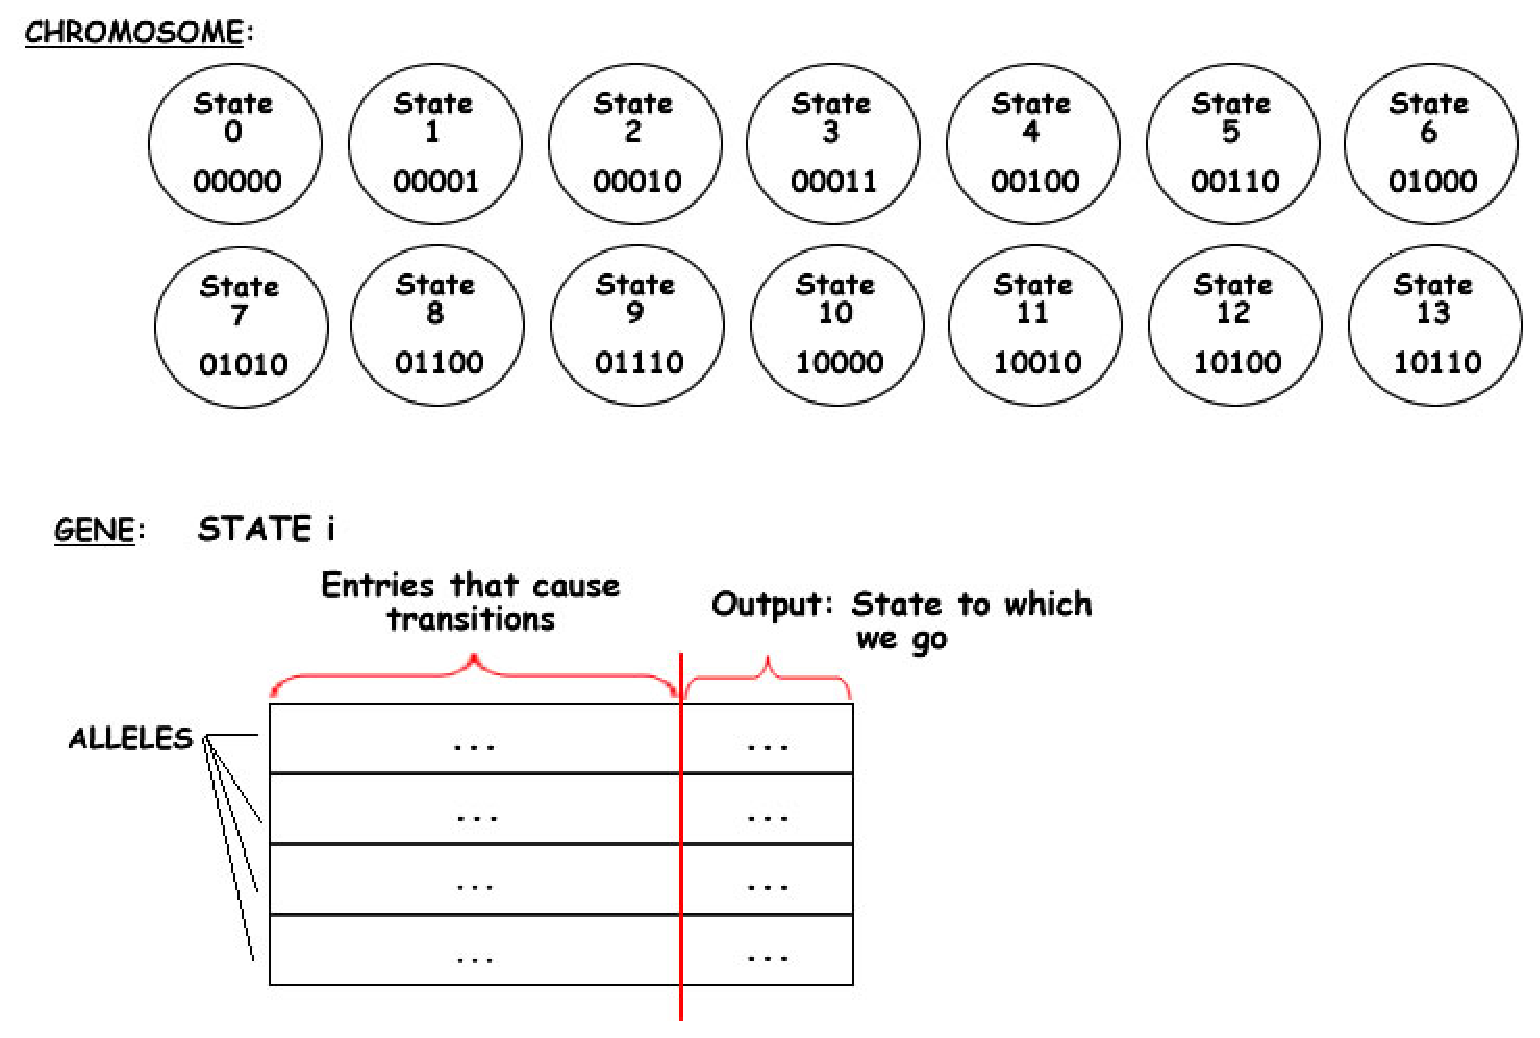
\includegraphics[scale=0.4]{imags/chromosome-fsm.eps}
\caption{Chromosome codification for the FSM evolution by means of a GA.
\label{fig:chromo_fsm}}
\end{center}
\end{figure}

The \textit{fitness function}, as usually in EAs, is the most important factor, since the algorithm performance strongly depends on it.
To calculate this function for one individual, the FSM represented in a chromosome is set as the AI of one agent which is placed in a game level, and then, it plays for getting its fitness value.
Two different schemes have been implemented:
\begin{itemize}
    \item \textit{mono-seed}: Every individual is tested in the same level (with the same difficulty) one time, until it passes the level, dies or gets stacked (do not get the end of the scenario on time). The length of the level and thus the time to complete it grow with the generations, being easier in the first generations and harder when the algorithm run advances. The aim is to improve the convergence. If the individuals in a generation do not get a good enough fitness on average, the level length and available time remain the same in the next generation.
    \item \textit{multi-seed}: Every individual is tested in 30 levels (with the same difficulty) generated randomly using different seeds, playing again until pass, die or get stacked. The fitness is computed considering the results of all the plays for an individual. The aim of this scheme is: 1) avoid the usual noise \cite{noisyfitness_EVO2012} present in this type of problems (videogames), i.e. it tries to get a fair valuation for an individual, since the same configuration could represent an agent which is very good sometimes and quite bad some others, due to the stochasticity of every play (regarding the agent's behaviour); and 2) get individuals prepared to a wide set of situations in every level and difficulty, since 30 levels should present a high amount of different scenarios and configurations.
\end{itemize}

Thus, there is a \textit{generic fitness} which has as restriction completely finish the level to be set to positive. On the contrary, individuals that have not finished the level start from the lowest fitness possible and their negativity is reduced according the behaviour during the level run. This generic fitness is a weighted aggregation, similar to the one implemented inside the simulator to assign the score, and which is based in the next values:
\begin{itemize}
\item {\em marioWinner}: is set to 1 if the agent finish the level.
\item {\em marioSize}: 0 if the agent is small, 1 if it is Big, and 2 if it is Fire.
\item {\em numKilledEnemies}: as the name suggest, is the number of killed enemies by the agent.
\item {\em numTotalEnemies}: number of total enemies during the level.
\item {\em cells}: number of cells passed by the agent.
\item {\em remainingTime}: time to finish the level.
\item {\em timeSpent}: time spent by the agent.
\item {\em coinsGathered}: number of gathered coins.
\item {\em totalCoins}: total coins appeared in the level.
\item {\em numCollisions}: number of times the agent has bumped with an enemy.
\item {\em numGatheredPowerUps}: number of mushrooms or flower the agent has picked up.
\item {\em causeOfDeath}: in case the agent is dead, this value is also taken into account in the fitness computation.
\end{itemize}

This fitness is considered as the result of the evaluation for the individuals in the mono-seed approach, meanwhile multi-seed considers a {\em hierarchical fitness}, where the population is ordered according the next criteria: 
First, taking into account the percentage of levels where the individuals have been stacked or fallen from a cliff. Then, they are ordered considering the average percentage of levels completed. Finally, the individuals are ordered by the average generic fitness obtained in the levels.

The considered operators in the GA are described in the following paragraphs. 
The {\em selection mechanism} considers the best individual and a percentage of the best ones, selected by tournament according to their fitness (generic or hierarchical, depending on the approach). Thus, when comparing two individuals in the multi-seed scheme, three values are considered in cascade: percentage of levels where the agent has been stacked or fallen in a gap, percentage of levels completed, and generic fitness.
The percentage of individuals to consider as parents follows two different schemes: in mono-seed it is low at the beginning and will be increased when the number of generations grows (to improve the convergence in the final generations); in multi-seed it is constant.

{\em Crossover} is performed considering the best individual of the present generation as one of the parents, and one of the individuals with positive fitness as the other parent. They generate a number of descendents which depends on the percentage of population to complete with the crossover. If there are not enough parents, we select the `less worse' individuals of those with negative fitness.
A uniform crossover has been used, i.e. each gene is randomly selected from one of the two parents.


The {\em Mutation operator} is slightly different from the usual one: after selecting a percentage of individuals to be mutated (mutation rate), various genes in each of these individuals are randomly selected to be mutated. Mutation is performed by randomly changing the output state for an input in the table.

Regarding the {\em replacement} to form the new population, there is a $1-elitism$ mechanism, so the best individual survives. The rest of the population is composed by the offspring generated in the previous generation, which was a percentage of the global population, and the rest of individuals being random ones, in order to increase the diversity, and thus, the exploration.
The percentage defined, in fact, is related to the number of random individuals, which is the complementary to the percentage of the generated offspring. This value is reduced with the generations in the mono-seed approach, as stated some paragraphs above. The aim is getting a high diversification factor in the first generations, i.e. an exploration phase, and reduce this factor when the best solutions arise (in some generations), changing to an exploitation phase. In multi-seed approach the percentage remains constant (quite small) because the fitness is much more representative of the individuals' quality, so the exploration has a lower significance.

%%%%%%%%%%%%%%%%%%%%%%%%%%%%%  EXPERIMENTS %%%%%%%%%%%%%%%%%%%%%%%%%%%%%%%%

\section{Experiments and Results}
\label{sec:experiments}

The aim of the proposed methods is to find good enough agents for completing any level in any difficulty, so in order to test these approaches, several experiments have been conducted.

As an initial step it was performed a hard fine-tuning stage (through systematic experimentation), in which several different values for the algorithms' parameters were tested, looking for the best configuration. 

In addition, in the experiments a wide analysis on the influence of these parameters was done, due to the difficulties that the algorithms found from level 5 onwards, as will be described in the next paragraphs.

It is important to remark that a single play of an agent could spend around 40-50 seconds on average (it depends on the level length and difficulty), because it must be played in real-time, not simulated. This fact means that a single evaluation for one individual in the multi-seed approach (30 plays) could take around 25 minutes in some levels. 

Moreover, when the experiments were conducted, it could be noticed that the most difficult levels strongly limited the algorithmic behaviour of the approaches, making it hard to converge and even ending the execution abruptly.
In addition to the high computational cost (one run may take several days), the huge size (in memory terms) of the structure that stores the individuals' FSM, can make the program finish due to a lack of memory. This structure grows exponentially during the run (new inputs and outputs are added to the tables in crossovers), so in levels higher than 4, the program frequently crashes.


% -------------------------------------------------------------------
\subsection{Mono-seed approach}

The first set of experiments were performed on a Phenom II X4 925 with 16GB RAM.
The main problem arose initially in levels higher than 5, where the memory limitations make the application crash. Thus, the global FSM structure implementation was redesigned to an optimal one, giving the chance to evolve agents in all the possible levels, but with a shorter number of generations than would be recommended.

The parameter analysis yielded the best configuration for the GA, whose values are presented in Table \ref{tab:params_monoseed}.

\begin{table} [htbp]
\caption{Optimal parameter values for mono-seed approach.
\label{tab:params_monoseed} }
\centering
{\footnotesize
\begin{tabular}{|l|l|}
\cline{2-2}
\multicolumn{1}{l|}{} & Optimal value \\ 
\hline
Population size & 1000 (difficulty 0) \\ 
Number of generations & 30 (difficulty 0) \\ 
Crossover percentage & 95\% \\ 
Mutation percentage & 2\% (individuals)\\ 
Mutation rate & 1\% (genes) \\ 
Percentage of random individuals & 5\% (decreased with the generations) \\
Fitness function & generic (aggregation) \\
\hline
\end{tabular}
}
\end{table}

The values in the table show that a small number of generations is required to get competent agents in difficulty level 0, along with a population size quite high since every individual is just tested once in this approach, so it is needed to ensure the evolution, yielding individuals which can complete the level. 
The population size was deeply studied, performing several runs for every configuration and considering when a successful agent was obtained for each difficulty level. The obtained results are plotted in Figure \ref{fig:population_monoseed}.
%
\begin{figure}
\begin{center}
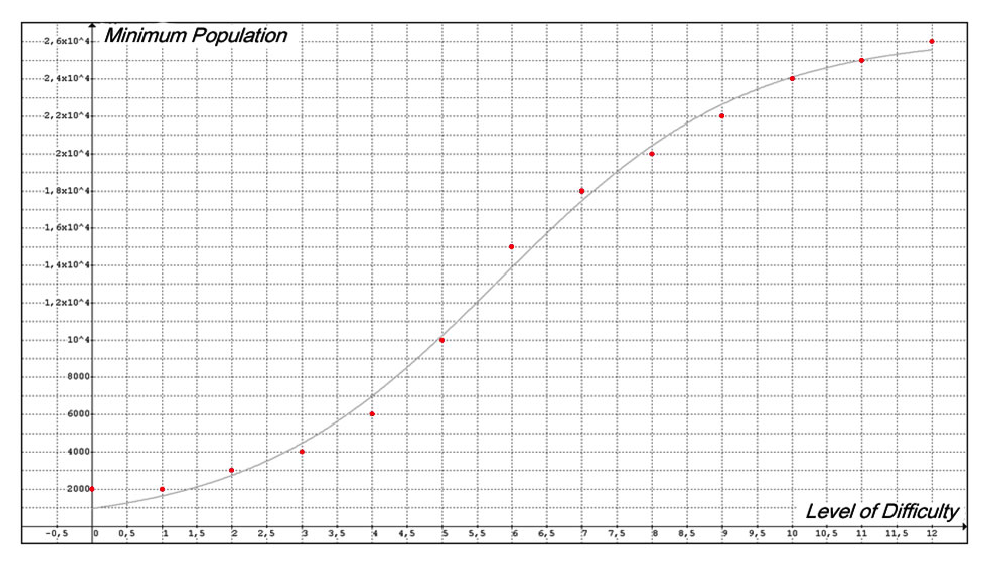
\includegraphics[scale=0.75]{imags/population_monoseed.eps}
\caption{Population size recommended for each difficulty level in mono-seed approach.
\label{fig:population_monoseed}}
\end{center}
\end{figure}
%
In this figure it can be seen the huge population sizes required to obtain competent agents in the most difficult levels, due to the evaluation criteria based in just one play per individual.

Moreover, Figure \ref{fig:time_memory_monoseed} presents the requirements in computation time and memory that a complete evolution (run of the algorithm) needed in every difficulty level. As it is shown, the algorithm is very exigent regarding machine resources.
%
\begin{figure}
\begin{center}
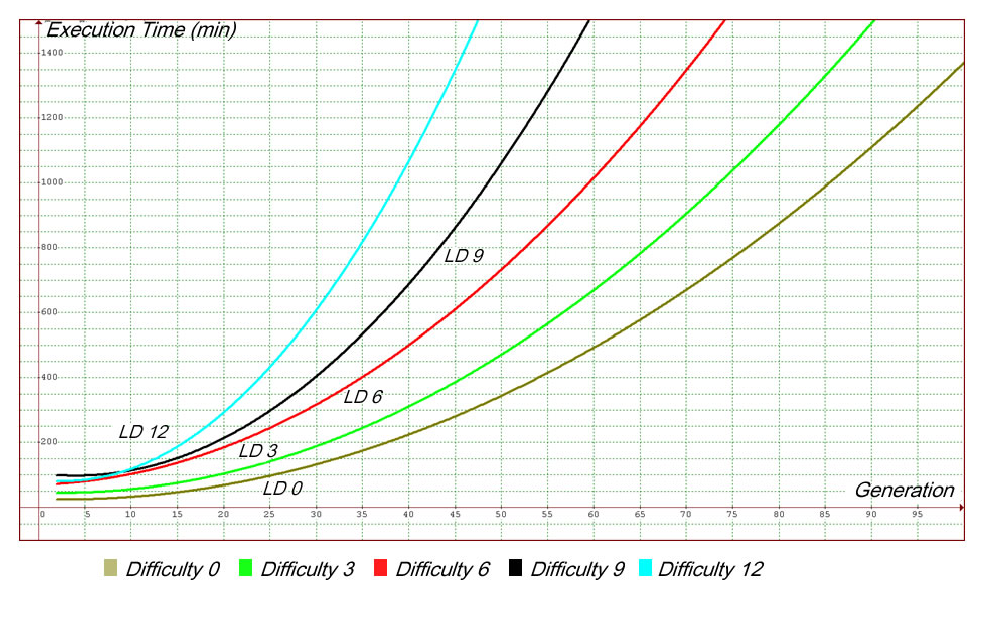
\includegraphics[scale=0.75]{imags/comp_time_monoseed.eps}
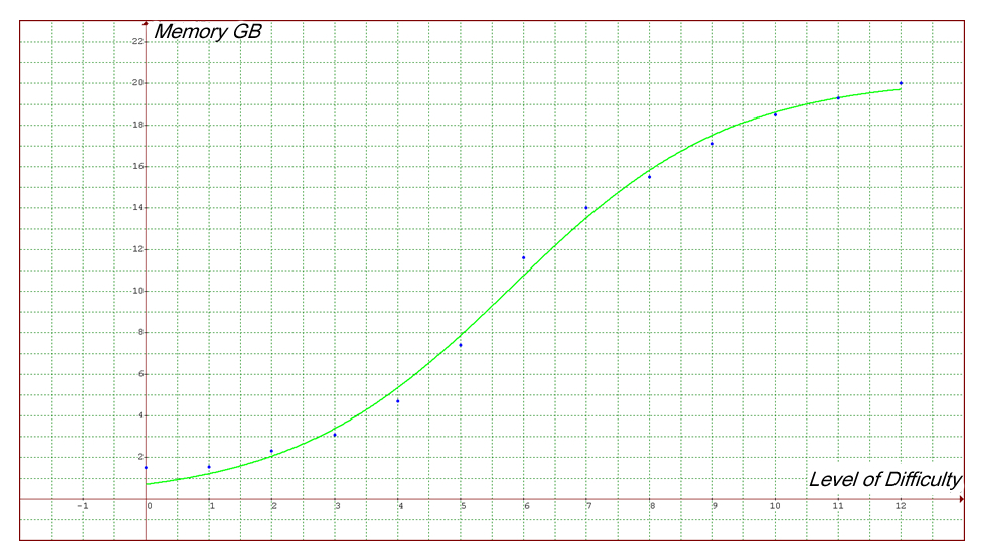
\includegraphics[scale=0.75]{imags/memory_monoseed.eps}
\caption{Run machine requirements: computation time (in minutes) and occupied memory (GB) for mono-seed approach.
\label{fig:time_memory_monoseed}}
\end{center}
\end{figure}

The fitness evolution (in difficulty 0) can be seen in Figure \ref{fig:maxfitness_monoseed}, where the maximum fitness value and the number of individuals with positive fitness (required to perform the crossover) are plotted. 
%
\begin{figure}
\begin{center}
\includegraphics[scale=0.27]{imags/max_fitness_monoseed.eps}
\caption{Maximum fitness in every generation, along with the number of individuals with positive fitness in mono-seed approach. Difficulty level 0.
\label{fig:maxfitness_monoseed}}
\end{center}
\end{figure}
%
It can be seen that the fitness grows with the generations, as expected in a GA, and there are always enough individuals with positive fitness to ensure the offspring generation.

The agents obtained with mono-seed approach are very good for the specific level (depends on the generation seed) and difficulty for which they were `trained', i.e. those which were set during the optimisation process. They also behave very well in different lengths (for the same level), since this grows with the generations, as commented in Section \ref{sec:FSMagent}.
However their behaviour is quite bad when the level generation seed or the difficulty are changed.

% -------------------------------------------------------------------
\subsection{Multi-seed approach}

Due to the problems of previous experiments, multi-seed study was conducted on a better computer, an Intel Core i7-920 processor with 32GB RAM. However the memory problem still remained. 
Thus, as a first improvement the number of states where reduced to 12, by deleting those considered as non-useful (in Table \ref{tab:FSMstates}): State 8 (no action is done) and State 11 (Mario jumps and crouch, since this actions are not possible simultaneously in this implementation of Infinite Mario).
With this change, it was possible to evolve competent agents from difficulty levels 0 to 4, which are, in turn, enough for the Gameplay competition.

As previously stated, in this approach, every individual is evaluated in 30 different levels, with different random seeds and level type (exterior, subterranean or castle), but with the same length and associated difficulty.

Moreover, in order to get a better computation time, we profited the architecture of the machine, so the fitness evaluation was divided in four parallel threads (four levels at a time), getting an improvement of around four times.

The optimal values for this approach are shown in Table \ref{tab:params_multiseed}.

\begin{table} [htbp]
\caption{Optimal parameter values for multi-seed approach.
\label{tab:params_multiseed} }
\centering
{\footnotesize
\begin{tabular}{|l|l|}
\cline{2-2}
\multicolumn{1}{l|}{} & Optimal value \\ 
\hline
Population size & 2000 (difficulty 4)\\ 
Number of generations & 500 (difficulty 4)\\ 
Crossover percentage & 95\% \\ 
Mutation percentage & 2\% (individuals)\\ 
Mutation rate & 1\% (genes)\\ 
Percentage of random individuals & 5\% (constant)\\ 
Fitness function & hierarchical \\
\hline
\end{tabular}
}
\end{table}

These values show a number of generations smaller than in mono-seed approach for difficulty level 4 (which was set to 6000 in that case), since the individuals here are evaluated in 30 different levels against just one in that approach, so the adaptation is much more higher and thus, it is not necessary to have a very high amount of individuals.

However, the time spent and memory required are even higher than before, as it can be seen in Figure \ref{fig:time_memory_multiseed}, which shows the analysis of memory and computation time consumed in the evolution until difficulty 4. 
%
\begin{figure}
\begin{center}
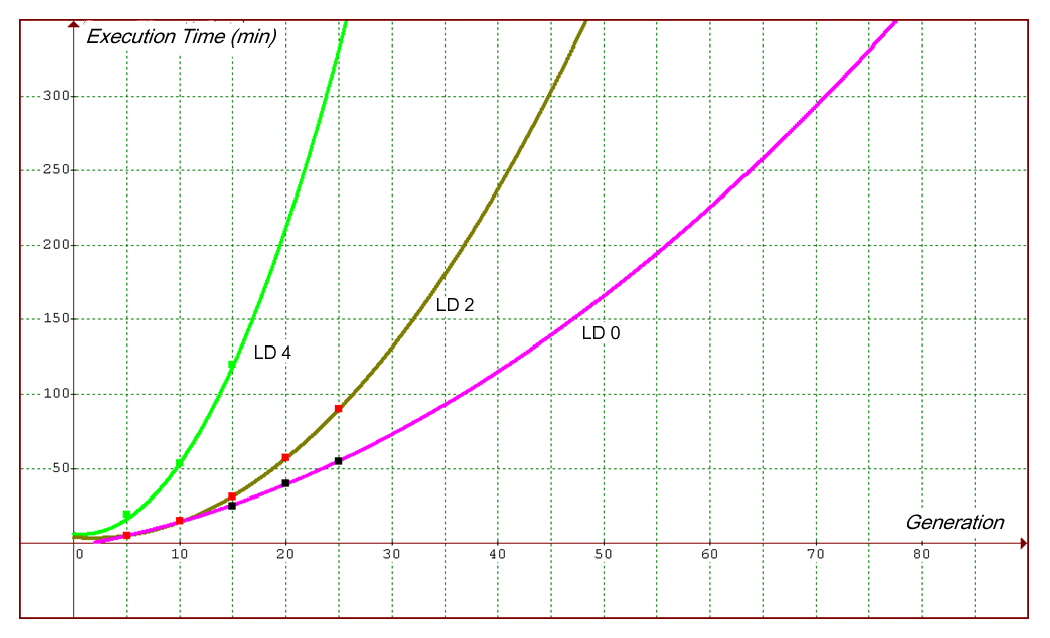
\includegraphics[scale=0.70]{imags/comp_time_multiseed.eps}
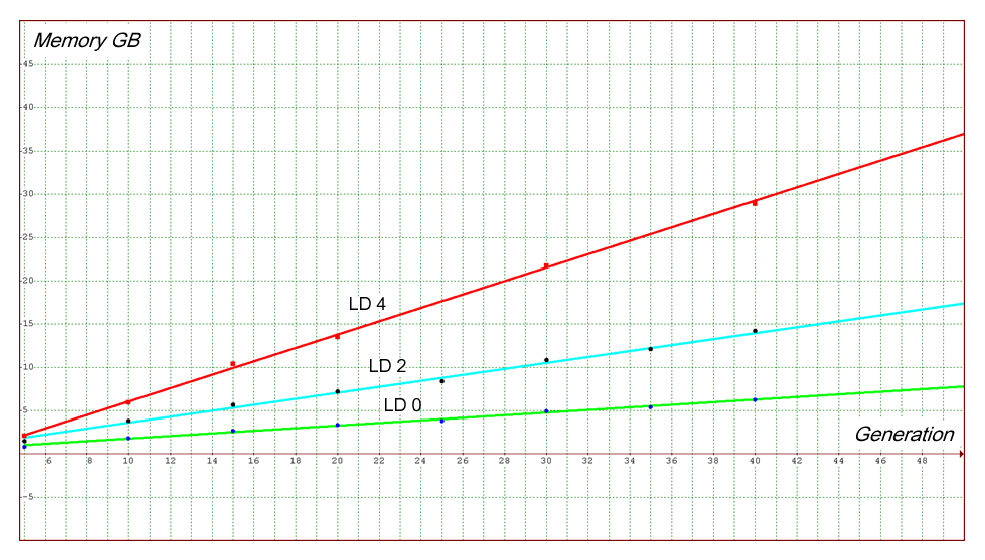
\includegraphics[scale=0.75]{imags/memory_multiseed.eps}
\caption{Run machine requirements: computation time (in minutes) and occupied memory (GB) for multi-seed approach.
\label{fig:time_memory_multiseed}}
\end{center}
\end{figure}
%
The time consumption was logical, due to the number of evaluations to perform per individual. The memory requirements is explained since every table in each chromosome grows when new inputs (situations) arise in the game, so the must be considered in the FSM. In 30 plays and in quite difficult levels, this number grows exponentially.

However, the agents obtained with multi-seed approach are able to complete (almost) any scenario in every level of difficulty for which they have been optimised.

Some examples of the obtained evolved FSM-based agents can be seen in action (in a video) from the next urls:
\begin{itemize}
    \item \textit{Difficulty level 1 (completed)}: \url{http://www.youtube.com/watch?v=6Pj6dZCE070}
    \item \textit{Difficulty level 2 (completed)}: \url{http://www.youtube.com/watch?v=gtfuY-L0WDA}
    \item \textit{Difficulty level 3 (completed)}: \url{http://www.youtube.com/watch?v=qQVQ43sWwYY}
    \item \textit{Difficulty level 12 (stacked)}: \url{http://www.youtube.com/watch?v=zNGfBApX7sk}
\end{itemize}

The last one was evolved for some generations (not all the desired) in that level of difficulty, due to the commented problems, so it cannot complete this hard level in the simulator. However, as it can be seen, it is quite good in the first part of the play. Thus, if we could finish the complete evolution process in this difficulty level we think the agent could complete any possible level.

%LT -> Tipo de escenario. Escenario 0: superficie, escenario 1: subterr�neo, escenario 2: castillo
%LD -> Dificultad del nivel. Valores entre 0 y 12
%LL -> Longitud del nivel. Valor de 26 a $2^(31)-1$
%LS -> Semilla aleatoria de generaci�n de nivel. Valor de 0 a $2^(31)-1$
%

%%%%%%%%%%%%%%%%%%%%%%%%%%%%% CONCLUSIONS %%%%%%%%%%%%%%%%%%%%%%%%%%%%%%%%

\section{Conclusions and Future Work}
\label{sec:conclusions}

This work presents two different approaches of evolutionary-based autonomous agents for playing the videogame Super Mario Bros. They have been implemented using Finite State Machine (FSM) models evolved by means of a Genetic Algorithm (GA), using different evaluation schemes: mono-seed and multi-seed approaches, and two different fitness functions.
Both approaches have been implemented inside a simulator named Mario AI, based in the so-called Infinite Mario Bros, which was implemented for the International Mario AI Competition. The proposed agents were focused, in principle to participate in the Gameplay Track of that competition.

Several experiments have been conducted to test the algorithms and a deep analysis has been performed in each case, in order to set the best configuration parameters for the GA. However some problems have arisen such as the high memory requirements, which have made it difficult to complete the optimisation process in some cases.

Even so, very competent agents have been obtained for the difficulty levels 0 to 4 in both approaches, which are, in turn, enough for the Gameplay competition requirements.

In the comparison between the approaches, mono-seed can yield excellent agents for the level where they were `trained' (evolved), having a quite bad behaviour in a different level. Multi-seed takes much more computation time and has higher memory requirements, but the agents it yields are very good playing in any level of the considered difficulty during the evolution. All these agents play much better than an expert human player and can complete the levels in a time impossible to get for the human.

Since this is a novel research scope for the authors, several future lines of work are opened, starting with the resolution of the commented memory problem. A redesign of the GA's chromosome structure could be useful in this sense.
We definitely think that if it is possible to completely evolve a population of agents with the multi-seed scheme, the best of them might complete any level.
Moreover, some other algorithmic proposals should be tested, such as a reduction in the number of individuals in the population, along with a change in the selection, crossover and mutation mechanisms to control the required balance between exploration and exploitation in GAs.

Another line of research could be the consideration of a high-level expert knowledge in the FSM. For instance each state should be based in principles proposed by \cite{SuperMario_rulebased}. That means the agents should be not designed according a fixed set of states, but the specific necessities that it should solve in every situation. This solution could reduce the search space and increase the possibility to solve harder levels.

\begin{acknowledgements}
This work has been supported in part by the P08-TIC-03903 project awarded by the Andalusian Regional Government, the FPU Grant 2009-2942 and the TIN2011-28627-C04-02 project, awarded by the Spanish Ministry of Science and Innovation.
\end{acknowledgements}


% BibTeX users please use one of
\bibliographystyle{spbasic}      % basic style, author-year citations
%\bibliographystyle{spmpsci}      % mathematics and physical sciences
%\bibliographystyle{spphys}       % APS-like style for physics
%\bibliography{}   % name your BibTeX data base

% Non-BibTeX users please use
\begin{thebibliography}{00}

\bibitem{EAs_Back96}
B\"ack, T., \emph{Evolutionary algorithms in theory and practice}, Oxford University Press, 1996.

\bibitem{SuperMario_Astar}
R. Baumgarten, \emph{Mario AI A* agent},
http://www.doc.ic.ac.uk/~rb1006/projects:marioai.

\bibitem{SuperMario_rulebased}
Bojarski, S., Bates-Congdon, C., \emph{REALM: A Rule-Based Evolutionary Computation Agent that Learns to Play Mario}. In: Proceedings of the 2011 IEEE Symposium on Computational Intelligence and Games (CIG 2011), IEEE Press, pp. 83--90, 2011. 

\bibitem{FSM_Booth}
Booth, T.L., \emph{Sequential Machines and Automata Theory}, John Wiley and Sons, Inc., New York, 1st edition, 1967.

\bibitem{ControllingBot_CEC2010}
Esparcia-Alc{\'a}zar A I, Mart�nez-Garc\'{\i}a A I, Mora A M, Merelo J J, Garc\'{\i}a-S{\'a}nchez P. Controlling bots in a first person shooter game using genetic algorithms. In \emph{Proc. 2010 IEEE Congress on Evolutionary Computation (CEC 2010)}, July 2010, pp. 1--8.

\bibitem{Genebot_CEC11}
Fern�ndez-Ares, A., Mora, A.M., Merelo, J.J., Garc�a-S�nchez, P., Fernandes,
  C.:
\newblock Optimizing player behavior in a real-time strategy game using
  evolutionary algorithms.
\newblock In: Evolutionary Computation, 2011. CEC '11. IEEE Congress on. (2011)
   2017--2024

\bibitem{GAs_Goldberg89}
Goldberg D.E., Korb B., Deb K., \emph{Messy genetic algorithms: motivation, analysis, and first results}, Complex Systems, 3(5), pp. 493--530, 1989.

\bibitem{potfields_starcraft}
Hagelb\"ack, J., \emph{Potential-Field Based navigation in StarCraft}. In: Proceedings of the 2012 IEEE Symposium on Computational Intelligence and Games (CIG 2012), IEEE Press, pp. 388--393, 2012. 

\bibitem{optimalRTS}
Jang, S.H., Yoon, J.W., Cho, S.B., \emph{Optimal strategy selection of non-player character on real time strategy game using a speciated evolutionary algorithm}. In: Proceedings of the 5th IEEE Symposium on Computational Intelligence and Games (CIG'09), IEEE Press, pp. 75--79, 2009.

\bibitem{laird2001using}
Laird, J.E, \emph{Using a computer game to develop advanced AI}.
  Computer, 34(7), pp. 70--75, 2001.

\bibitem{Pac-MAnt_CIG2010}
Mart�n, E., Mart�nez, M., Recio, G., Saez, Y., \emph{{Pac-mAnt}: Optimization based on ant colonies applied to developing an agent for Ms. Pac-Man}. In Proc. 2010 IEEE Conference on Computational Intelligence and Games (CIG 2010), IEEE Press, pp. 458--464, 2010.

\bibitem{Mora_Unrealbot_EVO2010}
Mora, A.M., Montoya, R., Merelo, J.J., Garc�a-S�nchez, P., Castillo, P.A.,
  Laredo, J.L.J., Mart�nez, A., Esparcia, A.I.:
\newblock Evolving bot {AI} in {U}nreal.
\newblock In et~al., C.D.C., ed.: Applications of Evolutionary Computing, Part
  I. Volume 6024 of LNCS., Springer (2010)  170--179

\bibitem{cooperativebots_CIG2010}
Mora, A.M., Moreno, M.A., Merelo, J.J., Castillo, P.A., Garc�a-Arenas, M.I., Laredo, J.L.J., \emph{Evolving the cooperative behaviour in {Unreal}\texttrademark~ bots}. In Proc. 2010 IEEE Conference on Computational Intelligence and Games (CIG 2010), IEEE Press, pp. 241--248, 2010.

\bibitem{noisyfitness_EVO2012}
Mora, A.M., Fern�ndez-Ares, A., Merelo, J.J., Garc�a-S�nchez, P., \emph{Dealing with noisy fitness in the design of a RTS game bot}. In Proc. Applications of Evolutionary Computing: EvoApplications 2012, LNCS, vol. 7248, Springer, pp. 234--244, 2012.

\bibitem{SuperMario_playerexperience}
Pedersen, C., Togelius, J., Yannakakis, G., \emph{Modeling Player Experience in Super Mario Bros}. In Proc. 2009 IEEE Symposium on Computational Intelligence and Games (CIG'09), IEEE Press, pp 132--139, 2009.

\bibitem{MTCS_PacMan}
Pepels, T., Windans, H.M., \emph{Enhancements for Monte-Carlo Tree Search in Ms Pac-Man}. In Proc. 2012 IEEE Conference on Computational Intelligence and Games (CIG 2012), IEEE Press, pp. 265--272, 2012.

\bibitem{tactics_evolutionary_learning}
Ponsen, M., Munoz-Avila, H., Spronck, P., Aha, D.W., \emph{Automatically generating game tactics through evolutionary learning}. AI Magazine, 27(3), pp. 75--84, 2006.

\bibitem{SuperMario_levelgeneration}
Shaker, N., Nicolau M., Yannakakis, G.N., Togelius, J., O\textquoteright neill, M., \emph{Evolving Levels for Super Mario Bros Using Grammatical Evolution}. In Proc. 2012 IEEE Symposium on Computational Intelligence and Games (CIG 2012), IEEE Press, pp 304--311, 2012.

\bibitem{Agent_Smith_CEC2009}
Small, R., Bates-Congdon, C. \emph{Agent {S}mith: Towards an evolutionary
  rule-based agent for interactive dynamic games}. In Proc. 2009 IEEE Congress on Evolutionary Computation (CEC'09), pp. 660--666, 2009.

\bibitem{evolutionary_learning-offline}
Spronck, P., Sprinkhuizen-Kuyper, I., Postma, E., \emph{Improving opponent intelligence through offline evolutionary learning}. International Journal of Intelligent Games and Simulation, 2(1), pp. 20--27, 2003.

\bibitem{starcraft_bayesianmodel}
Synnaeve, G., Bessi�re, P., \emph{A Bayesian Model for RTS Units Control applied to StarCraft}. In Proc. 2011 IEEE Symposium on Computational Intelligence and Games (CIG 2011), IEEE Press, pp 190--196, 2011.

\bibitem{SuperMario_Togelius}
Togelius, J., Karakovskiy, S., Koutnik, J., Schmidhuber, J., \emph{Super Mario
  evolution}. In Proc. 2009 IEEE Symposium on Computational Intelligence and Games (CIG'09), IEEE Press, pp 156--161, 2009.

\end{thebibliography}

\end{document}
% end of file template.tex

